\section{Q1: Mean face}
\label{subsec:Q1_meanface}
\begin{figure}[htbp]
	\centering
	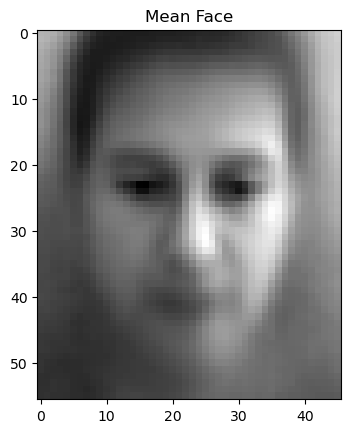
\includegraphics[width=0.4\linewidth]{image/q1_meanface.png} 
	\caption{Mean face of training data}
	\label{fig:q1_meanface}
\end{figure}

\section{Q1,3: Confusion matrix}
\label{subsec:Q13_cm}
\begin{figure}[htbp]
	\centering
        \begin{subfigure}[t]{0.3\linewidth}
		\centering
	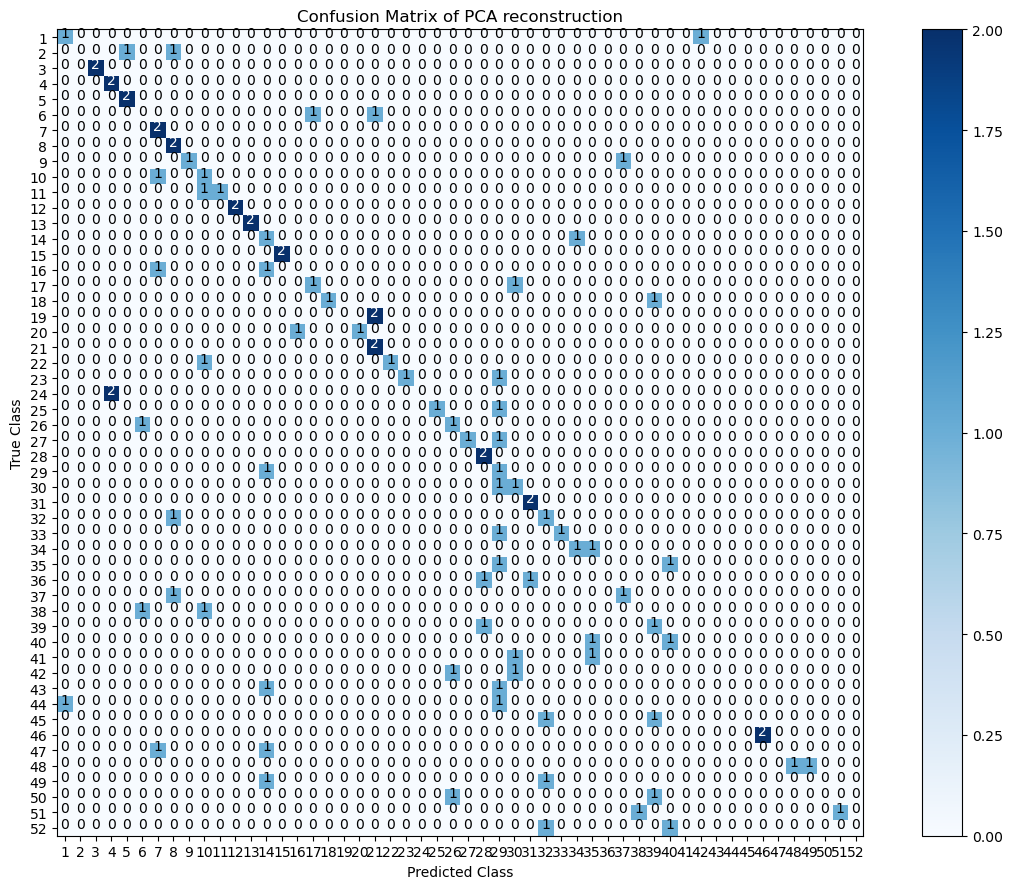
\includegraphics[width=\linewidth]{image/q1_cm.png}
	\caption{Confusion matrix of PCA}
	\label{fig:q1_cm}
        \end{subfigure}
    \quad
        \begin{subfigure}[t]{0.3\linewidth}
        \centering
        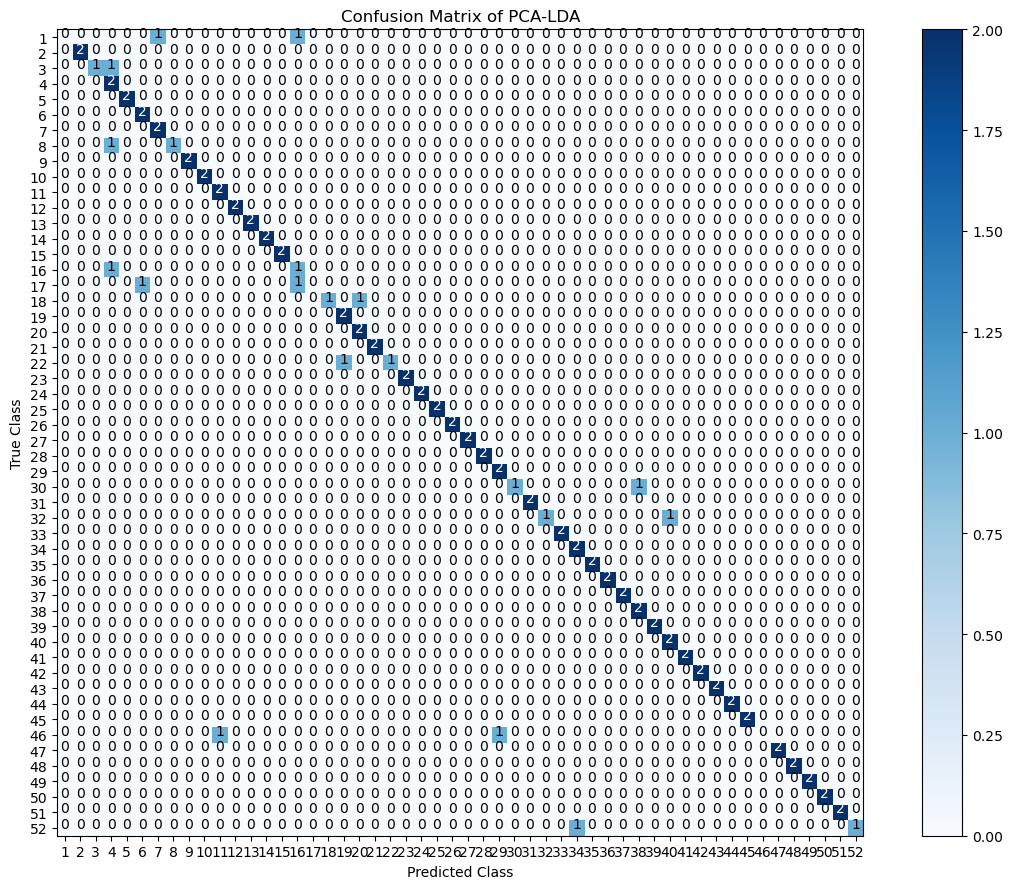
\includegraphics[width=\linewidth]{image/q3_1_cm.png} % Seems better to move to Appendix,,
	\caption{Confusion matrix of PCA-LDA}
	\label{fig:q3_1_cm}
        \end{subfigure}
    \quad
        \begin{subfigure}[t]{0.3\linewidth}
        \centering
        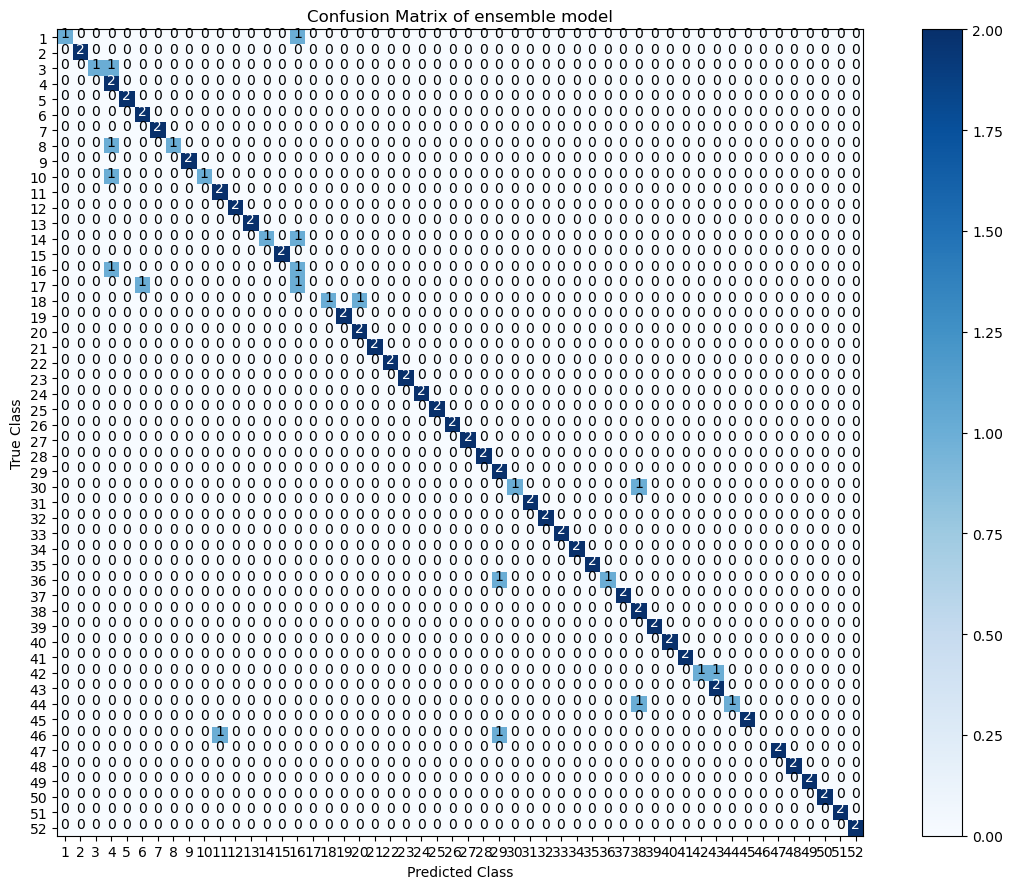
\includegraphics[width=\linewidth]{image/q3_2_cm.png} % Seems better to move to Appendix,,
	\caption{Confusion matrix of Emsenble model}
	\label{fig:q3_1_cm}
        \end{subfigure}
    \label{fig:cm}
\end{figure}

As shown in \cref{fig:cm}, confusion matrix of PCA has much more off-diagonal elements than PCA-LDA and Ensemble model. This shows that the prediction is much more successful using PCA-LDA and Ensemble model than PCA. Also, Ensemble model has slightly less off-diagonal elements than PCA-LDA. This indicates Ensemble model is more accurate in classification than the original model. 
% \cref{fig:q3_1_cm} is the confusion matrix of PCA-LDA classification result. As most of prediction result is on the diagonal entry, it indicates that most of prediction is successful. We take a closer look at success and failure cases. \cref{fig:q3_success} shows successfully predicted cases. Despite the different angles of the faces, the model infer the class accurately. \cref{fig:q3_fail} is failure cases. It seems that the prediction failed because of the similar glasses and face expression.

%-----
\newpage
\section{Q1,3: Prediction examples}
\label{subsec:Q13_eg}
\begin{figure}[htbp]
	\centering
        \begin{subfigure}[t]{0.4\linewidth}
        \centering
        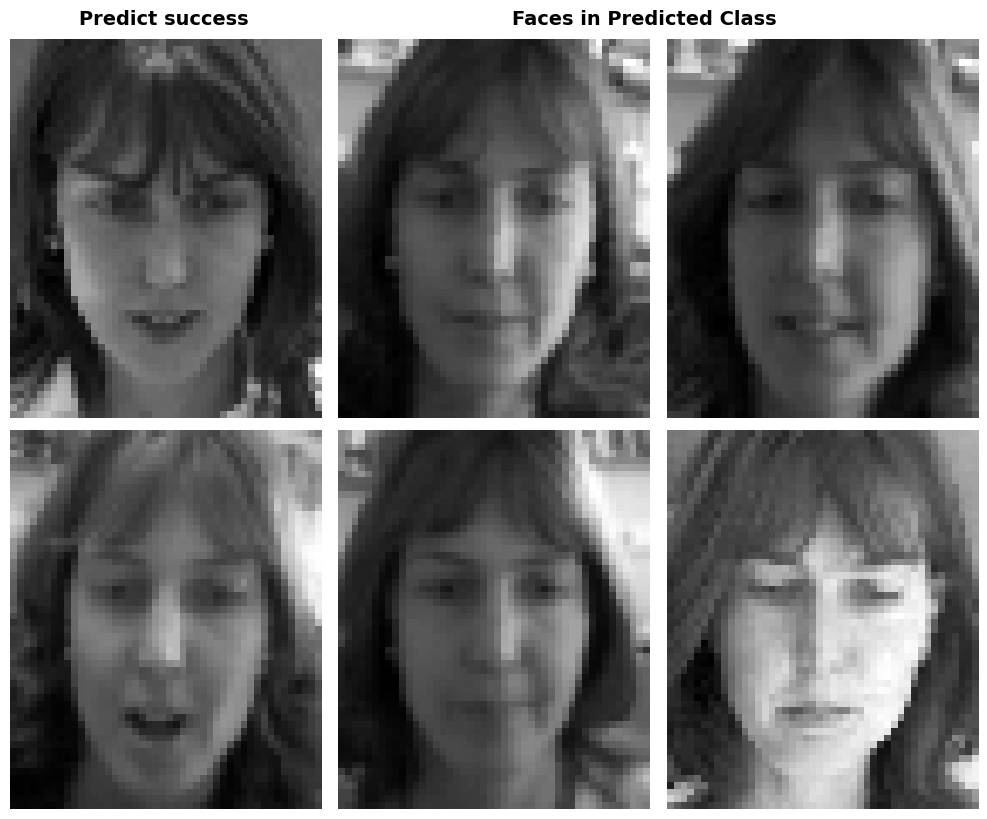
\includegraphics[width=\linewidth]{image/q1_success.png}
	\caption{PCA classification success example}
	\label{fig:q3_success}
        \end{subfigure}
    \quad
        \begin{subfigure}[t]{0.4\linewidth}
        \centering
        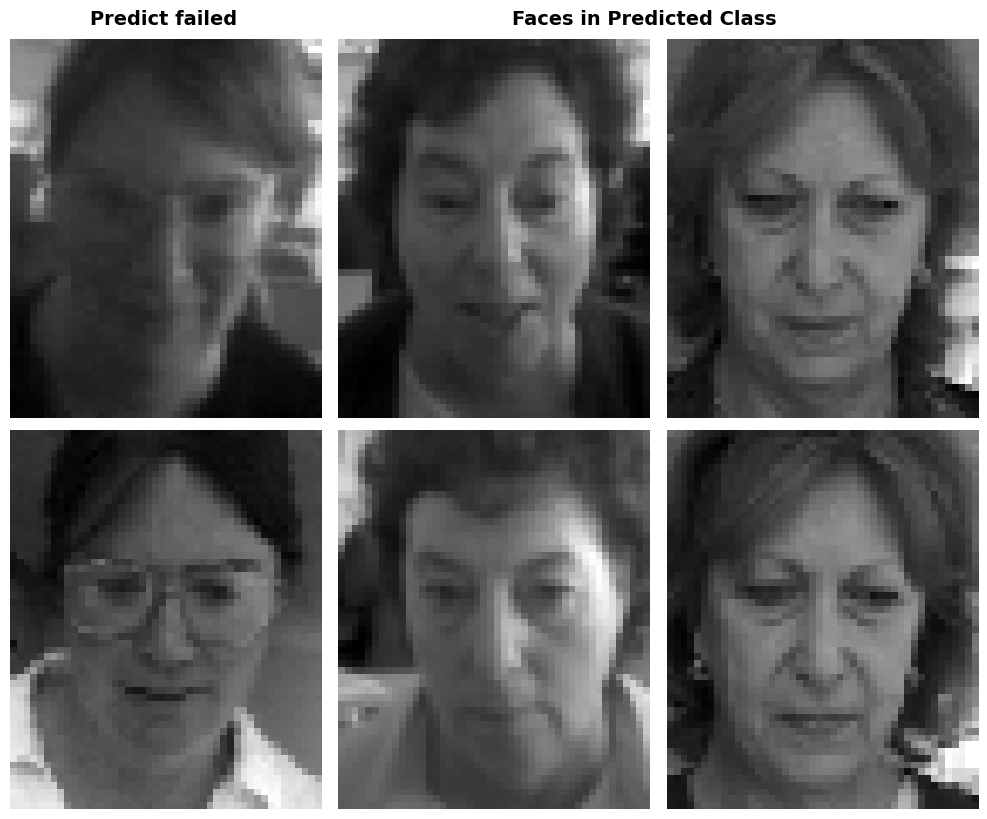
\includegraphics[width=\linewidth]{image/q1_fail.png}
	\caption{PCA classification failure example}
	\label{fig:q3_fail}
        \end{subfigure}
    \quad
	\begin{subfigure}[t]{0.4\linewidth}
	\centering
	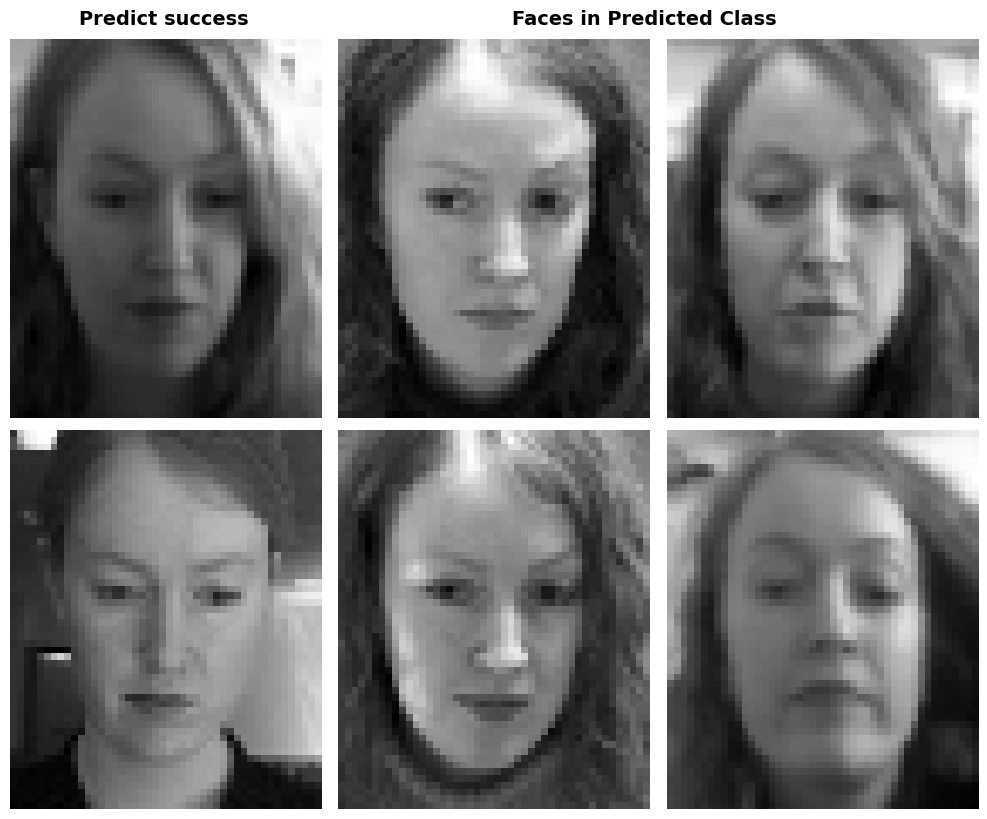
\includegraphics[width=\linewidth]{image/q3_success.png}
	\caption{PCA-LDA classification success example}
	\label{fig:q3_success}
        \end{subfigure}
    \quad
        \begin{subfigure}[t]{0.4\linewidth}
	\centering
	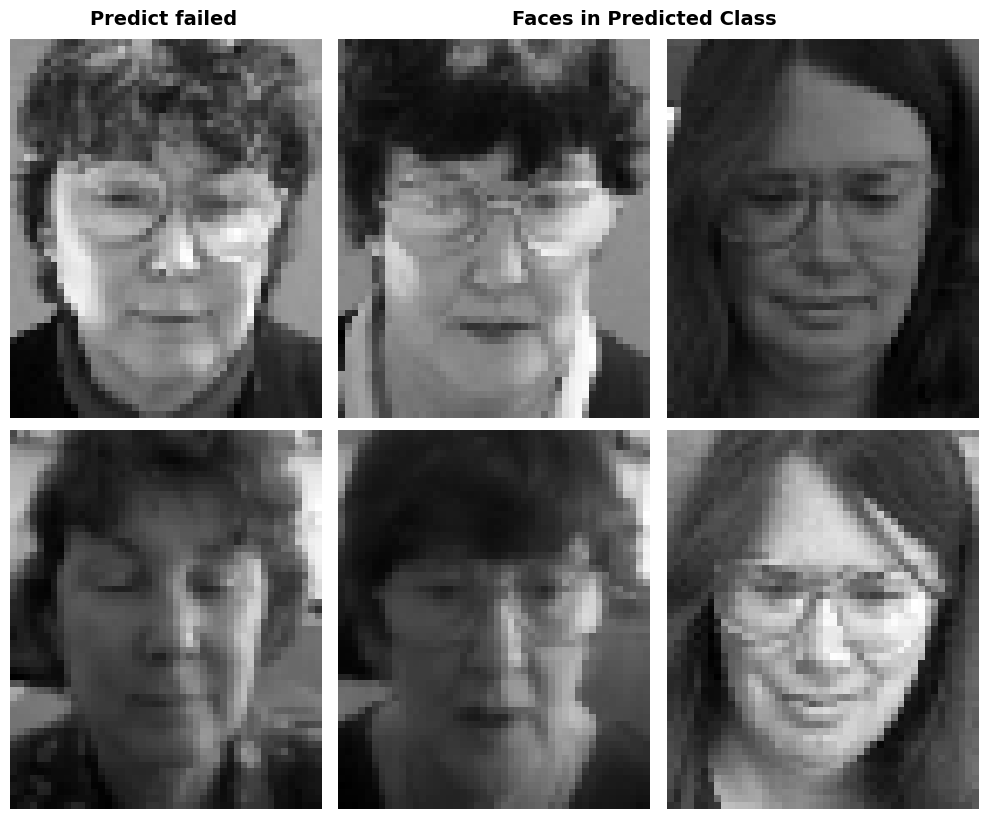
\includegraphics[width=\linewidth]{image/q3_fail.png}
	\caption{PCA-LDA classification failure example}
	\label{fig:q3_fail}
    \end{subfigure}
\end{figure}
Above images shows successful and failure examples of classification using PCA and PCA-LDA. If we take a closer look at successful cases, the model infer the class accurately despite different angles of face. This may because the model can generalize well across different angles of the face. For failure cases, the prediction appears to have failed because the glasses and facial expressions are similar.

\section{Q4: Generative and Discriminative Subspace Learning}
\label{subsec:Q4}
\label{sec:intro}
Below is the objective function for generative and discriminative subspace learning. Our goal is to find $W$ that maximizes $J(W)$
\begin{equation}
	J(W) = \alpha W^TSW+(1-\alpha) \frac{W^TS_bW}{W^TS_wW}
	\label{eq:pca_lda_2}
\end{equation}
\cref{eq:pca_lda_2} can be changed as \cref{eq:pca_lda_3} since $W^TW=I$. (This is because, $W$ is a projection matrix, hence $W^TW$ indicates re-projection after projection to the subspace. Therefore, projected vector returns to itself after applying $W^TW$.)
\begin{equation}
	J(W) = \alpha \frac{W^TSW}{W^TW}+(1-\alpha) \frac{W^TS_bW}{W^TS_wW}
	= \frac{W^T(\alpha S + (1-\alpha)S_b)W}{W^T(\alpha I + (1-\alpha)S_w)W}
	\label{eq:pca_lda_3}
\end{equation}
If we keep the denominator constant, the problem we have to solve changes to the problem to maximize the numerator. Let the denominator $k(constant)$ and use Lagrange-multiplier. (\cref{eq:denominator})
\begin{equation}
	W^T(\alpha I + (1-\alpha)S_w)W = k
	\label{eq:denominator}
\end{equation}
\begin{equation}
	L(W,\lambda)=W^T(\alpha S + (1-\alpha)S_b)W
	+ \lambda(k-W^T\alpha I + (1-\alpha)S_w)W)
	\label{eq:lagrange}
\end{equation}
To get the solution, each partial derivatives of $L(W,\lambda)$ with respect to $W$ and $\lambda$ must be 0.
\begin{equation}
	\frac{\partial L}{\partial W} = 2*W(\alpha S+(1-\alpha)S_b
	-\lambda(\alpha I+(1-\alpha)S_w))=0
	\label{eq:partial_W}
\end{equation}
\begin{equation}
	\frac{\partial L}{\partial \lambda} = k - W^T(\alpha I+(1-\alpha)S_w)W=0
	\label{eq:partial_lambda}
\end{equation}
\cref{eq:partial_lambda} is satisfied from our assumption of the denominator. Now, the only thing we have to consider is \cref{eq:partial_W}. If we organize \cref{eq:partial_W}, we can get \cref{eq:solution}.
\begin{equation}
	(\alpha S+(1-\alpha)S_b)W = \lambda (\alpha I + (1-\alpha)S_w)W
	\label{eq:solution}
\end{equation}
If $\alpha I + (1-\alpha)S_w$ is invertible, the equation becomes as below.(\cref{eq:final})
\begin{equation}
	(\alpha I + (1-\alpha)S_w)^{-1}(\alpha S+(1-\alpha)S_b)W = \lambda W
	\label{eq:final}
\end{equation}
Since $\lambda$ is some constants, we can regard \cref{eq:final} as a eigenvector-eigenvalue problem where W is an eigenvector matrix and lambda is an eigenvalue matrix.

\section{Q5: Test result's confusion matrix and success/failure cases }
\label{subsec:Q5-1}
The optimal parameters determined for the random forest through experiments are $N=250$, $D=8$, and $\text{splitnum}=10$. With this configuration, each real-time executable weak learner—axis-aligned and two-pixel tests—each was trained 10 times. The confusion matrix results in \cref{fig:app-q5-6} represent the best test accuracy among the 10 repetitive train results.

\begin{figure}[htbp]
	\centering
	\begin{subfigure}[t]{0.4\linewidth}
		\centering
		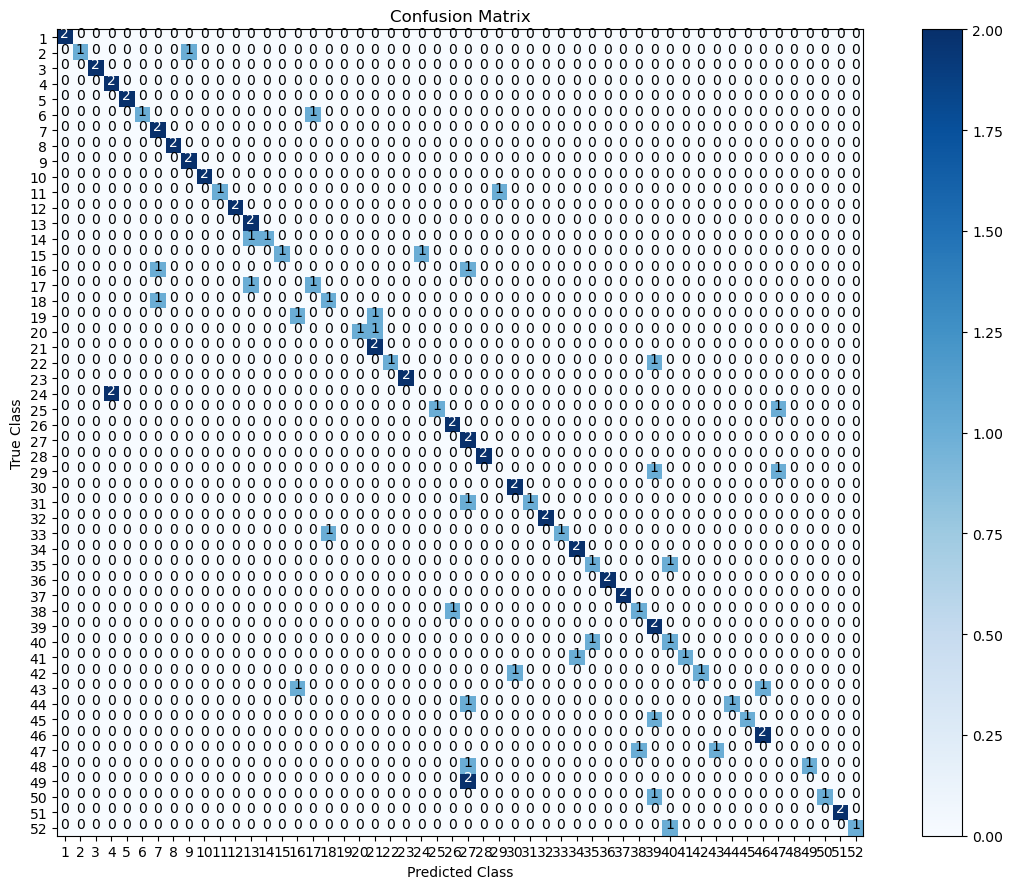
\includegraphics[width=\linewidth]{image/q5-fig6.png}
		\caption{Axis-aligned weak learner, test accuracy=0.644}
		\label{fig:q5-fig6}
	\end{subfigure}%
	\quad
	\begin{subfigure}[t]{0.4\linewidth}
		\centering
		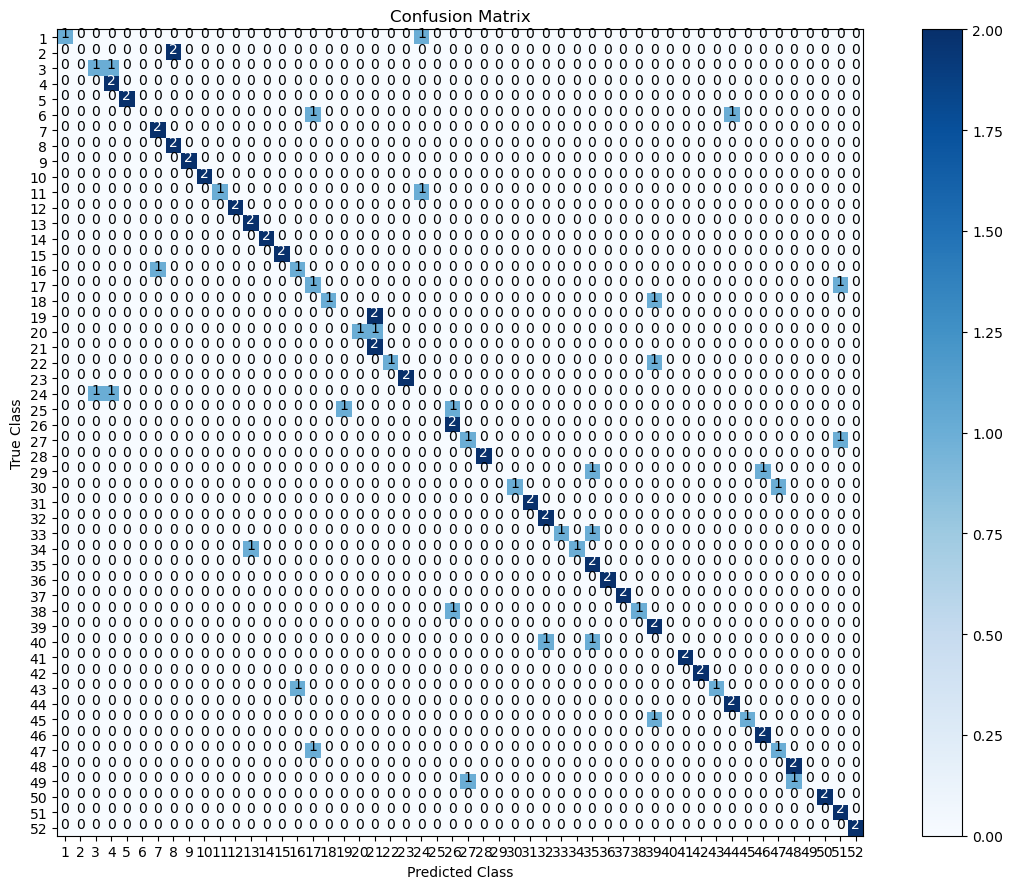
\includegraphics[width=\linewidth]{image/q5-fig8.png}
		\caption{Two-pixel test weak learner, test accuracy=0.692}
		\label{fig:q5-fig8}
	\end{subfigure}
	\caption{Confusion matrix of optimal cases ($N=250$, $D=8$, and $\text{splitnum}=10$)}
	\label{fig:app-q5-6}
\end{figure}

Additionally, the example success and failure cases based on the confusion matrix results above are shown in \cref{fig:app-q5-2}, \cref{fig:app-q5-3}, \cref{fig:app-q5-4}, \cref{fig:app-q5-5}. Compared to the success cases, the failure cases show a higher similarity between the failed image and the predicted class, meaning that our model is reasonable.
\begin{figure}[htbp]
	\centering
	\begin{subfigure}{0.45\linewidth}
		\centering
		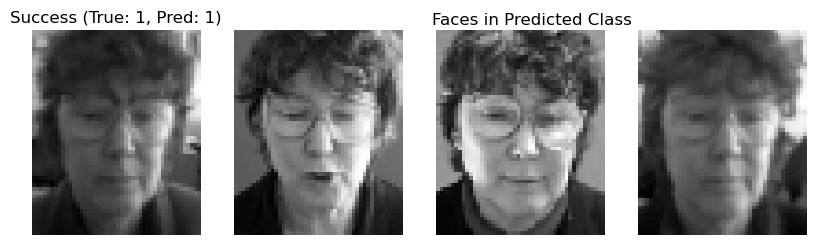
\includegraphics[width=\linewidth]{image/q5-app/q5-axis-succ1.png}
	\end{subfigure}%
	\quad
	\begin{subfigure}{0.45\linewidth}
		\centering
		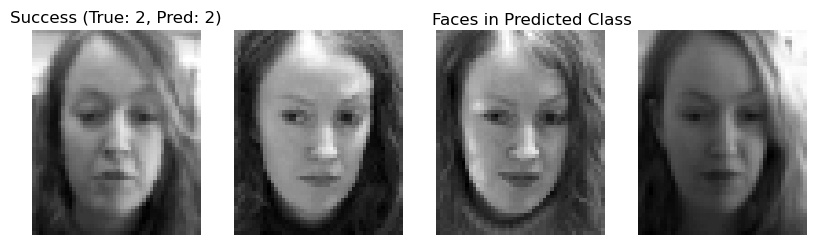
\includegraphics[width=\linewidth]{image/q5-app/q5-axis-succ2.png}
	\end{subfigure}
	\caption{Axis-aligned weak learner: Example success case}
	\label{fig:app-q5-2}
\end{figure}
\begin{figure}[htbp]
	\centering
	\begin{subfigure}[t]{0.45\linewidth}
		\centering
		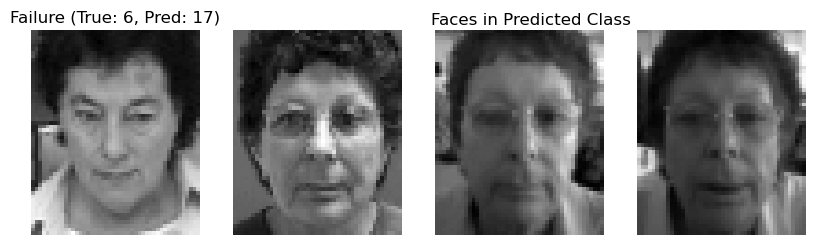
\includegraphics[width=\linewidth]{image/q5-app/q5-axis-fail1.png}
	\end{subfigure}%
	\quad
	\begin{subfigure}[t]{0.45\linewidth}
		\centering
		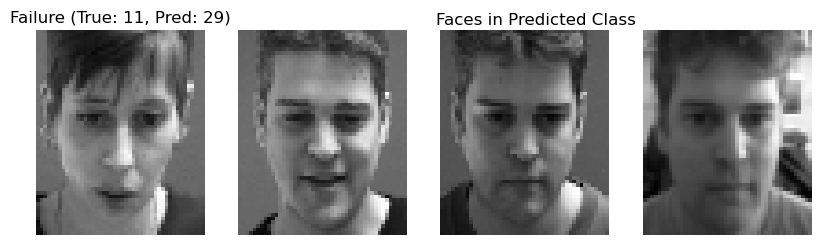
\includegraphics[width=\linewidth]{image/q5-app/q5-axis-fail2.png}
	\end{subfigure}
	\caption{Axis-aligned weak learner: Example failure case}
	\label{fig:app-q5-3}
\end{figure}

\begin{figure}[htbp]
	\centering
	\begin{subfigure}{0.45\linewidth}
		\centering
		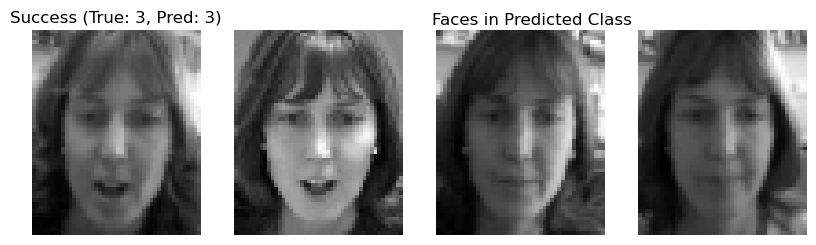
\includegraphics[width=\linewidth]{image/q5-app/q5-two-succ1.png}
	\end{subfigure}%
	\quad
	\begin{subfigure}{0.45\linewidth}
		\centering
		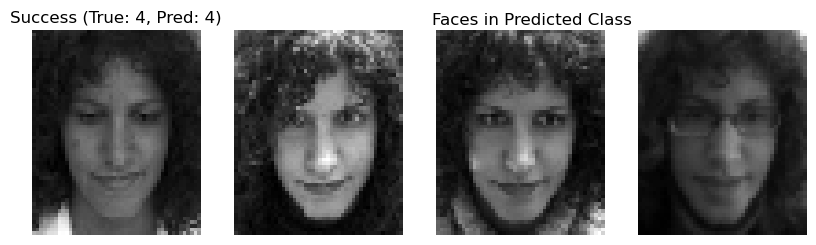
\includegraphics[width=\linewidth]{image/q5-app/q5-two-succ2.png}
	\end{subfigure}
	\caption{Two-pixel test weak learner: Example success case}
	\label{fig:app-q5-4}
\end{figure}
\begin{figure}[htbp]
	\centering
	\begin{subfigure}{0.45\linewidth}
		\centering
		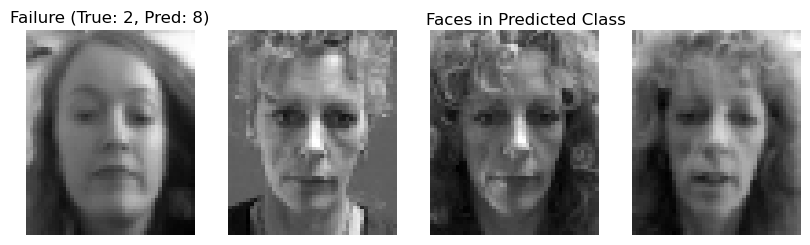
\includegraphics[width=\linewidth]{image/q5-app/q5-two-fail1.png}
	\end{subfigure}%
	\quad
	\begin{subfigure}{0.45\linewidth}
		\centering
		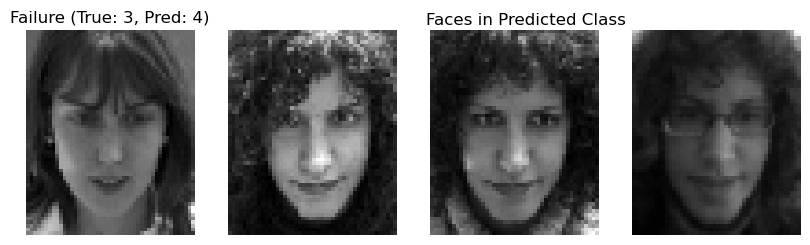
\includegraphics[width=\linewidth]{image/q5-app/q5-two-fail2.png}
	\end{subfigure}
	\caption{Two-pixel test weak learner: Example failure case}
	\label{fig:app-q5-5}
\end{figure}

\section{Q5: Visualization of random forest's information gain process}
\label{subsec:Q5-2}
Random forests utilize the entropy-based information gain method to reduce the diversity of classes within the nodes as they move down to the lower nodes. To illustrate the execution of this algorithm in our code, we have traced the path down the left child nodes of a single tree and represented the results in the histograms below. Each histogram corresponds to the left node of the previous figure, and the result \cref{fig:app-q5-1} align with our expectations.

\begin{figure}
	\centering
	\begin{subfigure}{0.33\linewidth}
		\centering
		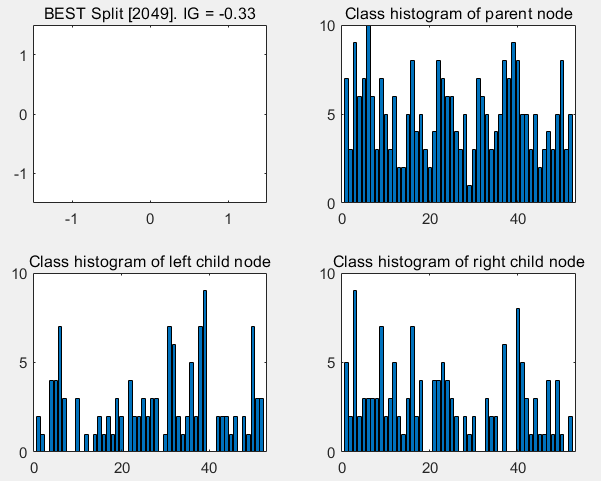
\includegraphics[width=\linewidth]{image/q5-app/hist1.png}
		\caption{Top node (depth=1)}
	\end{subfigure}%
	\hfill
	\begin{subfigure}{0.33\linewidth}
		\centering
		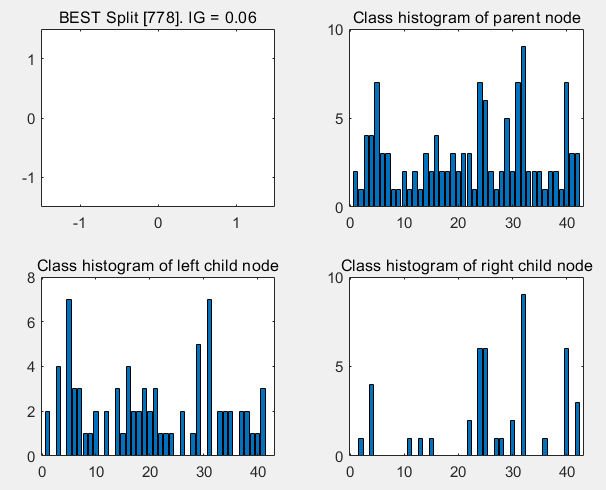
\includegraphics[width=\linewidth]{image/q5-app/hist2.png}
		\caption{depth=2}
	\end{subfigure}
	\hfill
	\begin{subfigure}{0.33\linewidth}
		\centering
		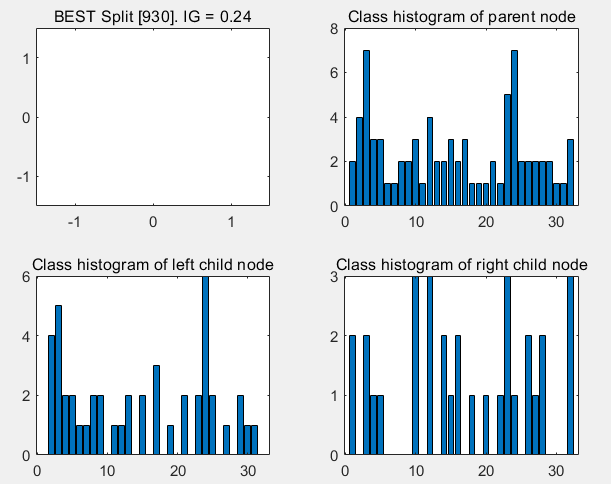
\includegraphics[width=\linewidth]{image/q5-app/hist3.png}
		\caption{depth=3}
	\end{subfigure}
	
	\begin{subfigure}{0.33\linewidth}
		\centering
		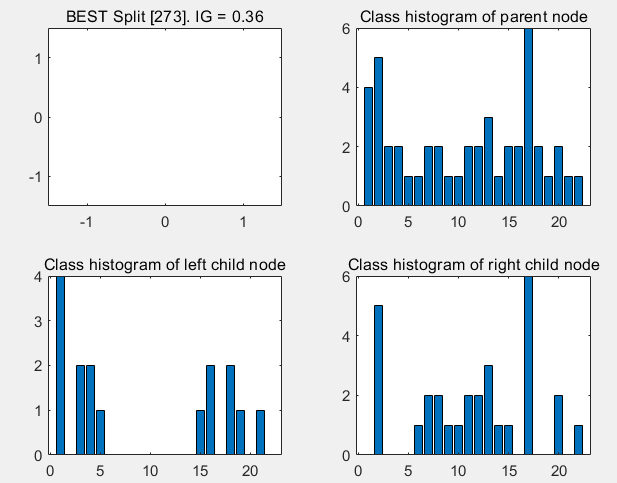
\includegraphics[width=\linewidth]{image/q5-app/hist4.png}
		\caption{depth=4}
	\end{subfigure}%
	\hfill
	\begin{subfigure}{0.33\linewidth}
		\centering
		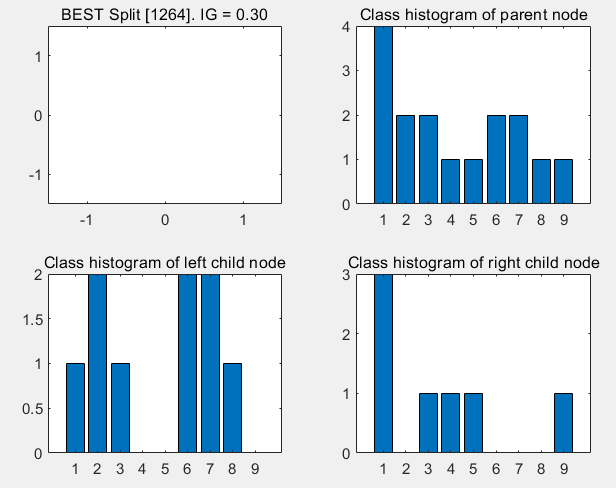
\includegraphics[width=\linewidth]{image/q5-app/hist5.png}
		\caption{depth=5}
	\end{subfigure}
	\hfill
	\begin{subfigure}{0.33\linewidth}
		\centering
		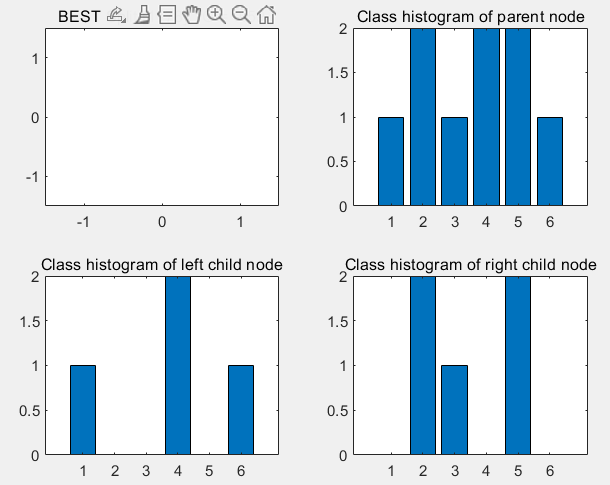
\includegraphics[width=\linewidth]{image/q5-app/hist6.png}
		\caption{Leaf (depth=6)}
	\end{subfigure}
	\caption{Visualization of random forest's information gain process}
	\label{fig:app-q5-1}
\end{figure}